\section{Künstliche Neuronale Netze}%
\label{sec:ann}

\begin{frame}{Künstliches Neuron}
  \begin{minipage}{.65\textwidth}
    \begin{tikzpicture}[->, >=stealth, thick, scale=.8]
      \node [circle split,draw,rotate=90] (z) at (0, 0) {\rotatebox{-90}{$\displaystyle\sum$} \nodepart{lower} \rotatebox{-90}{$\sigma(z)$}};
      \foreach \i in {5,...,1} {
        \node (x-\i) at (-7, 4.5+1.5*-\i) {\(x_{\i}\)};
        \path (x-\i) edge node[above] {\(w_{\i}\)} (z);
      }
      \node (y) at (4, 0) {\(a\)};
      \path (z) edge (y);
      \node (b) at (0, 2.5) {\(b\)};
      \draw (b) -- (z);
    \end{tikzpicture}
  \end{minipage}%
  \begin{minipage}{.35\textwidth}
    \uncover<2->{
      \begin{flushright}
        \begin{tabular}{cl}
          \toprule
          \(\mathbf{x}\)  & Inputvektor\\
          \(\mathbf{w}\)  & Gewichtsvektor\\
          \(b\)  & Bias\\
          \(z\)  & Zwischensumme \(\left(\sum\right)\)\\
          \(\sigma(x)\)  & Aktivierungsfunktion\\
          \(a\)  & Aktivierung/ Output\\
          \bottomrule
        \end{tabular}
      \end{flushright}
    }
  \end{minipage}

  \only<3>{
    \[z = \sum_{i}x_{i}w_i + b = \mathbf{xw} + b\]

    {\centering\(\Rightarrow z\) wird für spätere Parameteroptimierung benötigt\par}
  }
\end{frame}

\begin{frame}{Aktivierungsfunktion \(\sigma(x)\)}
  \begin{minipage}{.45\textwidth}
    \(\Rightarrow\) Es gibt eine Vielzahl verschiedener Aktivierungsfunktionen für unterschiedliche Problemstellungen, für uns soll jedoch lediglich die \textbf{Sigmoid-Funktion} relevant sein:

    \vspace{1cm}

    \[\sigma(x) = \frac{1}{1 + e^{-x}}\]
  \end{minipage}\hfill%
  \begin{minipage}{.5\textwidth}
    \only<2>{
      \begin{tikzpicture}
        \begin{axis}[width=\textwidth, mlineplot, samples=50, ymin=-.1, ymax=1.1, domain=-10:10, title=Sigmoid-Funktion, xlabel=\(x\), ylabel=\(\sigma(x)\)]
          \addplot{1/(1+exp(-x))};
        \end{axis}
      \end{tikzpicture}
    }
  \end{minipage}

\end{frame}

\begin{frame}{Architektur eines Neuronalen Netzwerks}
  \def\layersep{2.5cm}
  \begin{center}
    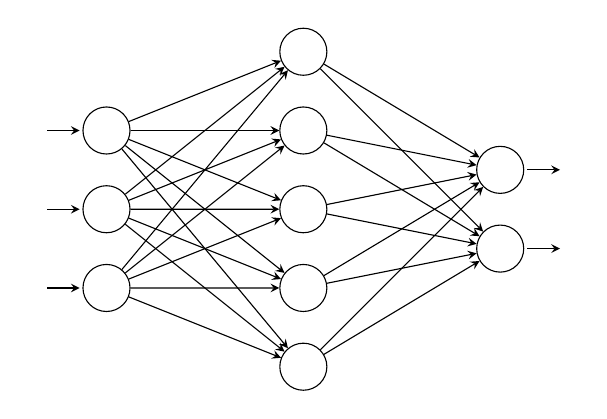
\begin{tikzpicture}[->, >=stealth]
      \tikzstyle{every pin edge}=[<-,shorten <=1pt]
      \tikzstyle{neuron}=[circle,draw,minimum size=17pt,inner sep=0pt]
      
      % Draw the input layer nodes
      \foreach \y in {1,...,3}
      \node[neuron, pin=left:] (I-\y) at (0,-\y) {};

      % Draw the nodes for the second hidden layer
      \foreach \y in {1,...,5}
      \path[yshift=(5cm - 3cm)/2] node[neuron] (H1-\y) at (\layersep,-\y cm) {};

      % Draw the output layer nodes
      \foreach \y in {1,...,2}
      \path[yshift=(2cm - 3cm)/2] node[neuron,pin={[pin edge={->}]right:}] (O-\y) at (2*\layersep,-\y cm) {};

      \foreach \source in {1,...,3}
      \foreach \dest in {1,...,5}
      \path (I-\source) edge (H1-\dest);

      \foreach \source in {1,...,5}
      \foreach \dest in {1,...,2}
      \path (H1-\source) edge (O-\dest);
    \end{tikzpicture}
  \end{center}

\end{frame}

%%% Local Variables:
%%% mode: latex
%%% TeX-master: "../präsentation"
%%% End:
